% Generic article-class manuscript (journal-agnostic). MT29 P2.
% Ported 2026-07-02 onto the reliability-commons paper-template pattern
% (../../reliability-commons/paper-template/):
% build with `make paper` (figures/*.R regenerate F1-F5 from the frozen result
% JSONs, `make bib` copies the portfolio shared.bib, latexmk -pdf compiles).
% Every number traces to research/results/MT29/{mt29_stage1_matched_yield_result.json,
% mt29_stage2_robustness_result.json} and the supplementary result JSONs cited inline.
\documentclass[11pt]{article}

\usepackage[utf8]{inputenc}
\usepackage[T1]{fontenc}
\usepackage[margin=1in]{geometry}
\usepackage{amsmath,amssymb}
\usepackage{graphicx}
\usepackage{booktabs}
\usepackage{tabularx}
\usepackage{siunitx}
\usepackage{caption}
\usepackage{subcaption}
\usepackage[numbers,round]{natbib}
\usepackage[hidelinks]{hyperref}
\usepackage{xcolor}
\usepackage{authblk}
\usepackage{microtype}

\newcommand{\TODO}[1]{\textcolor{red}{[TODO: #1]}}

\graphicspath{{figures/}}
\captionsetup{font=small,labelfont=bf}
\setlength{\parskip}{0.4em}

\title{The value of selective abstention in machine-learned stability
prediction tracks reference-data trustworthiness: a chemistry-stratified audit}
\author{Zeyu Fu\thanks{ORCID: \href{https://orcid.org/0009-0001-8329-0108}{0009-0001-8329-0108}.
  Correspondence: \href{mailto:fuzeyu09@gmail.com}{fuzeyu09@gmail.com}.} \\
  \small State Key Laboratory of Trauma and Chemical Poisoning, Institute of Combined Injury,
  Army Medical University, Chongqing, China}
\date{\today}

\begin{document}
\maketitle

\begin{abstract}
% 2026-07-16 revision: restructured takeaway-first / numbers-second / scope-last per
% (takeaway-first / numbers-second / scope-last); every number and claim below is unchanged from the
% pre-pass abstract (see paper.tex.bak-pre-readerpass), only the ordering changed.
\noindent The value of selective abstention in universal machine-learning interatomic potentials
(UIPs) is not uniform across chemistry, and --- our central claim --- its variation
\emph{tracks where the reference data is itself least trustworthy}: the effect is best read as a
\emph{diagnostic of reference-data trustworthiness}, not a deployable stratified allocator. We
establish this with a reusable, chemistry-stratified \emph{matched-yield audit protocol}: a
CPU-only, provenance-gated analysis any practitioner can run on published prediction files to
test whether abstention pays off more in some chemistries than others while controlling for
surfaced-yield artifacts. UIPs pre-screen candidate crystals for stability on the Matbench
Discovery benchmark, keeping only the most confident predictions and \emph{abstaining} on the
rest. Applying the protocol to cached predictions from four UIPs (CHGNet, M3GNet, MACE, ORB)
across six anion-class strata, we measure the stratum $\times$ coverage interaction in discovery
acceleration
% source: research/results/MT29/mt29_stage1_matched_yield_result.json (i.i.d. 48/60; shuffle 0/60; chgnet oxide-halide interaction_med 0.90092, CI [0.77394, 1.04197])
% source: results_expansion_2026-07-11/prototype_blocked_cis/mt29_prototype_blocked_ci_result.json (prototype-blocked 45/60; chgnet oxide-halide median 0.89624, CI [0.7419, 1.03792])
factor (DAF) under a common-absolute-yield control; it excludes zero in 45 of 60 cells under a
prototype-blocked bootstrap (48/60 i.i.d.), is oxide-anchored, and survives
leave-one-element-out, WBM-round, multiplicity, and alternative-stratification controls with a
clean shuffle null. Decomposed, the effect is a genuine precision advantage --- the CHGNet
oxide-vs-halide abstention gain is $+7.7$ precision points --- that DAF's base-rate
normalization then amplifies to the $+0.90$ headline (95\,\% CI $[0.74, 1.04]$); we report the
precision-point interaction as primary and the DAF number as its base-rate-amplified form. That
precision headroom sits exactly where UIP predictions disagree most with the MP2020-corrected
labels, which are also the benchmark's least reliable slice (correlated-$d$ oxides lacking a
consistent Hubbard-$U$ treatment).
% source: results_expansion_2026-07-14/mt29_roster_expansion_result.json (n_included_uip 32; MP+OMat positive-anchored 32/32; V3 perm_p 0.68153; orb_v3 ox-hal 0.6426)
Expanded to $44$ published-potential files ($43$ independent models after removing one
byte-identical duplicate), the oxide anchor is universal: CI-positive for
all $32$ modern UIPs, with no detectable generational difference ($p{=}0.68$, an honest null at
$n{=}16$ per arm rather than a demonstrated invariance); a prior Orb-v3
reversal was a self-inference artifact, corrected to $+0.64$. Scoping the claim: the
oxide-highest ordering is a pooled-evaluation property that does not transfer under a temporally
held-out split, and a stratum-aware knapsack allocator is falsified --- the clean shuffle null,
this generational equivalence, and the non-transfer are the protocol's built-in controls doing
their job, not the effect weakening, and what they jointly certify is an \emph{abstention-quality}
interaction at matched yield, not a model-ranking re-ordering.
\end{abstract}

\section{Introduction}

Evaluating the \emph{reliability} of universal machine-learning interatomic potentials (UIPs)
--- not their aggregate accuracy alone, but when their stability predictions can be trusted
enough to act on --- is now central to using them for materials screening. The primary
contribution of this paper is a reusable audit protocol for one concrete, decision-layer
reliability question --- does the value of selective abstention depend on chemistry? --- built
to be run, not just read: it operates CPU-only on any set of already-published UIP prediction
files, needs no retraining or GPU, and gates every reported number to a frozen, re-runnable
result. The answer is yes, and our central claim is what that dependence reveals: the value of
abstention is largest exactly where the underlying reference data is least trustworthy, so the
chemistry-stratified interaction is best read as a \emph{diagnostic of reference-data
trustworthiness} rather than as a deployable stratified abstention policy. The oxide-anchored
effect we report below is the worked demonstration of that protocol on a standard benchmark; its
honest nulls --- a clean shuffle control, no detectable generational difference, a falsified
stratum-aware allocator, and non-transfer under a temporal hold-out --- are not caveats bolted
on afterward but the very evidence that fixes the diagnostic (not allocator) reading: they are
the protocol's rigor made visible.

Matbench Discovery~\citep{riebesell2025} established universal machine-learning interatomic
potentials (UIPs) as the standard first-pass filter for thermodynamic stability: given a
relaxed candidate structure, a UIP predicts its formation energy, from which one computes a
predicted distance to the convex hull and labels the structure stable when that distance is
below zero. The benchmark's WBM test set~\citep{wang2021} contains $\sim$257k substitution-
generated structures with corrected DFT ground truth, and models such as
CHGNet~\citep{deng2023}, M3GNet~\citep{chen2022}, MACE~\citep{batatia2022mace}, and
ORB~\citep{neumann2024} now achieve useful stable/unstable discrimination across it.

A practitioner rarely needs to label every candidate. The operational question is
selection: which subset should be carried forward to expensive DFT or synthesis? Selective
abstention --- keeping only the highest-confidence predicted-stable structures and declining
to commit on the rest --- is the natural mechanism, and the absolute predicted hull margin
$|\hat{e}_{\mathrm{hull}}|$ is a free, model-native confidence signal. The relevant figure of
merit is the discovery acceleration factor (DAF), the precision of the surfaced shortlist
divided by the stratum's stable base rate, which is comparable across chemistries with
different base rates.\footnote{Per-stratum base DAF values trace to the frozen chemistry-yield
result; the halide baseline DAF present in that file is $3.005$ (CHGNet, coverage $0.5$), the
value used consistently here. A historical correction to this figure (from an earlier $4.42$)
is reflected in the frozen result, though its pre-freeze provenance trail is not preserved on
disk --- noted for transparency, as it does not affect any matched-yield interaction reported
here (all of which are recomputed from the same frozen result).}
The closest prior work on certifiable abstention for UIPs, PCM~\citep{pcm2026}, reports a
global risk AUC-ROC of 0.938 but does not stratify the value of abstention by anion chemistry
or apply a matched-yield control --- those are the contributions of the present study.

A companion selective-prediction study tested whether other confidence signals ---
isotonic-calibrated $p_{\mathrm{stable}}$ and cross-model ensemble disagreement --- beat the
free hull-margin baseline at matched coverage and matched stable-call yield, and found
that none did (0/12 model $\times$ coverage cells): hull margin itself was undefeated, i.e.\
``distance is all you need'' for this task. That result killed the wedge of a
learned/calibrated signal beating margin, not margin-based abstention itself, and motivates a
complementary, conditional question. Hull margin was shown to be a sufficient,
undefeated abstention signal in aggregate --- but is its benefit nonetheless
chemistry-dependent? If abstention buys far more in some anion classes than in
others at a matched surfaced-candidate budget, then a stratified abstention policy sharpens
an already-sufficient global one.

We contribute a reusable, matched-yield reliability-audit protocol for UIP abstention and apply
it to Matbench Discovery. Concretely, this paper makes three contributions.
\begin{itemize}
  \item We define genuine anion-class strata (electronegativity-priority assignment per
        formula) with materially different stable base rates (oxide $12.4\,\%$ vs.\ halide
        $27.8\,\%$) and measure the stratum $\times$ coverage interaction in DAF under a
        \emph{common-absolute-yield} control that reproduces the exact matched-yield semantics
        of that companion study, lifted to strata.
  \item We show the interaction is real (45/60 cells exclude zero under a prototype-blocked
        bootstrap; 48/60 under i.i.d.\ resampling), directional (oxides highest,
        halides/intermetallics lowest), and physically coherent, with a clean within-stratum
        shuffle-null (0/60).
  \item We harden it on two independent robustness axes --- leave-one-element-out (LOEO)
        and WBM-round (time-like) cross-splits --- and report transparently where statistical
        power, not the effect, runs out.
  \item We decompose the effect into a genuine precision advantage ($+7.7$ precision points,
        CHGNet oxide-vs-halide) and a base-rate-normalization factor that DAF folds in, report
        the precision-point interaction as primary, and trace the precision headroom to
        UIP--label disagreement on the benchmark's least trustworthy slice --- establishing the
        interaction as a diagnostic of reference-data trustworthiness.
\end{itemize}
We are explicit about scope throughout: the result is an abstention-quality
interaction at matched yield, read as a reference-data-trustworthiness diagnostic and not as a
deployable stratified allocator (which its own temporal-transfer and knapsack controls falsify),
and not as a claim that stratification re-orders the models, which it does not. The full scope
statement --- what this result establishes and what remains explicitly out of scope --- is given
in the Discussion (``Scope and what stays dead''); we flag the boundary here, before the Results,
so it need not be inferred retroactively. Figure~\ref{fig:f0} summarizes the protocol end to end, from the frozen,
provenance-gated prediction files through the two audit stages to the per-model-generation
verdict, with its two built-in controls --- the shuffle-null and the falsified stratum-aware
allocator --- shown as explicit checks.

\begin{figure}[t]
  \centering
  
\includegraphics[width=0.82\textwidth]{fig0_overview.pdf}
  \caption{The matched-yield reliability-audit protocol. Frozen, provenance/md5-gated UIP
  prediction files feed a chemistry-stratified matched-yield selection (anion-class strata,
  common absolute-yield budget $Y$), which is audited in two stages --- the Stage~1 stratum
  $\times$ coverage DAF interaction and the Stage~2 leave-one-element-out / WBM-round
  robustness gates --- to a verdict per model-generation claim. Two built-in controls (dashed)
  guard the audit: a shuffle-null that stays clean throughout, and a stratum-aware knapsack
  allocator that the protocol itself falsified.}
  \label{fig:f0}
\end{figure}

\paragraph{Notation.} Table~\ref{tab:notation} collects the recurring short-codes used
throughout, as a compact reference map; each term remains defined inline at its first use in the
running text below.

\begin{table}[h]
  \centering
  \small
  \caption{Notation used throughout this paper. Each term is also defined inline at first use;
  this table is a reference map, not a substitute for those definitions.}
  \label{tab:notation}
  \begin{tabularx}{\textwidth}{@{}l X@{}}
    \toprule
    Term & Meaning \\
    \midrule
    UIP & Universal machine-learning interatomic potential \\
    WBM & Matbench Discovery's substitution-generated test set, with corrected DFT ground truth \\
    DAF & Discovery acceleration factor: surfaced-shortlist precision $\div$ stratum stable base rate \\
    $\hat{e}_{\mathrm{hull}}$ & Predicted (signed) hull distance; $|\hat{e}_{\mathrm{hull}}|$ is the absolute margin used as the confidence signal \\
    $Y_{\mathrm{loose}}$, $Y_{\mathrm{tight}}$ & Common absolute surfaced-yield budgets (looser, tighter), held identical across strata \\
    $\mathrm{gain}_A - \mathrm{gain}_B$ & Stratum $\times$ coverage interaction: the matched-yield abstention-gain difference between strata $A$, $B$ \\
    LOEO & Leave-one-element-out robustness cross-split \\
    WBM round & Acquisition-round (time-like) robustness cross-split \\
    $p_{\mathrm{stable}}$ & Calibrated (or native-Gaussian) probability of stability \\
    SSCS & Worst-slab calibration gap, $\max_s|\mathrm{gap}_s|$ over strata $s$ \\
    \bottomrule
  \end{tabularx}
\end{table}

\section{Methods}

\paragraph{Data.} We use Matbench Discovery's public, on-disk cached artifacts: the
WBM summary ground truth (corrected formation energy and corrected hull distance per
structure identifier and chemical formula) and one cached predicted-formation-energy CSV per
UIP. After dropping rows with missing values and inner-joining all four model prediction sets,
$256{,}963$ structures remain. No network access, tokens, or downloads occur at run time;
all computation is CPU/pandas. The complete matched-yield interaction (Stage~1) and its two
robustness gates (Stage~2: leave-one-element-out and WBM-round, each with a $1000$-sample
bootstrap) reproduce byte-for-byte from the frozen prediction files in under five CPU-minutes
on a commodity laptop (measured $\sim$3\,min, single core, no GPU). A structure is \emph{stable}
when its corrected true hull
distance is below zero; the predicted hull distance is reconstructed as the true hull
distance plus the model's signed formation-energy error (a fixed-hull approximation validated
against a from-scratch phase-diagram recompute in the Discussion), and confidence is its absolute
value $|\hat{e}_{\mathrm{hull}}|$.

\paragraph{Anion-class strata.} Each formula is assigned to exactly one stratum by an
electronegativity-priority rule: halide $>$ oxide $>$ chalcogenide (S/Se/Te) $>$ pnictide
(N/P/As/Sb/Bi) $>$ intermetallic (all-metal) $>$ other (remaining main-group). All six strata
contain at least $\sim$23k structures and exhibit genuinely different stable base rates,
which is what makes DAF (base-rate-normalised) the appropriate cross-stratum metric.

\paragraph{Matched-yield abstention gain (the companion-study control).} To eliminate the
surfaced-candidate-yield confound that killed the unstratified wedge, we fix a \emph{common
absolute yield budget} $Y$: the same integer number of surfaced predicted-stable structures
in every stratum within a split. Per model we set $Y_{\mathrm{loose}} = \min$ over usable
strata of the total called-stable count, and $Y_{\mathrm{tight}} = Y_{\mathrm{loose}} // 2$.
Within each stratum we rank called-stable structures by confidence, take the top-$Y$, and
define the abstention gain as
\[
  \mathrm{gain} \;=\; \mathrm{DAF}(\text{top } Y_{\mathrm{tight}})
                    \;-\; \mathrm{DAF}(\text{top } Y_{\mathrm{loose}}),
\]
with $Y$ identical across strata. Because both the surfaced count and its change are held
fixed across strata, any surviving cross-stratum difference is an abstention-quality-by-
chemistry effect, not a yield-count artifact.

\paragraph{Interaction, bootstrap, and null.} The stratum $\times$ coverage interaction for a
stratum pair $(A,B)$ is $\mathrm{gain}_A - \mathrm{gain}_B$, evaluated per model. We bootstrap
within strata ($n_{\mathrm{boot}} = 1000$, seed $20260621$) and report the median and the
95\,\% percentile CI; a cell ``fires'' when its CI excludes zero. A shuffle/permutation
null control was committed ex ante in a dated pre-analysis design memo (written
hours before Stage-1 ran): it permutes the confidence signal within each
stratum's called-stable set, so abstention selects a random top-$Y$ and the gain should
vanish; we require this shuffle-null to be clean (near-zero firing) under every split.
Because WBM is generated by elemental substitution into shared prototypes, called-stable
structures are not independent within a stratum; we therefore additionally compute every
Stage-1 CI with a \emph{prototype-blocked} bootstrap that resamples
structural-prototype clusters with replacement within each stratum (block $=$ WBM
AFLOW prototype label), and adopt the blocked CIs as primary. All other quantities
(budgets, base rates, DAF points) are identical to the i.i.d.\ run and reproduce it
byte-for-byte.

\paragraph{Robustness gates.} Two independent cross-splits harden the Stage-1 interaction.
\emph{(i) Leave-one-element-out (LOEO):} drop every structure whose formula contains a
target element $E$ and recompute --- for the most common anion (O), the dominant cations
(Ni, Al, Ge, Cu, Fe, Sn, Si), and the stratum-defining anion-formers (F, S, N, P), giving 12
splits. \emph{(ii) WBM round:} restrict to each WBM acquisition round $r$ (parsed from
the round number embedded in each structure's identifier), a time-like distribution-shift axis,
giving 5 splits. Thin strata are guarded by minimum-row ($500$) and minimum-called-stable
($40$) thresholds and dropped from a split if below threshold. The general direction and
kill criterion for this robustness gate were committed ex ante in
a dated pre-analysis design memo (21:00, hours before Stage-1 ran); the exact operational
SUCCESS threshold --- the interaction excludes zero for a majority of cells in a majority of
LOEO splits and a majority of rounds, with the shuffle-null clean throughout --- is
documented in a Stage-2 analysis-protocol log written in the
same analysis session as the Stage-2 results it reports, not registered before Stage-1.

\section{Results}

\subsection{Matched-yield abstention lifts DAF most in oxides}

Figure~\ref{fig:f1} shows DAF at the looser and tighter yield budgets for every
(stratum, model) pair. Across models, abstaining (moving from $Y_{\mathrm{loose}}$ to the
tighter $Y_{\mathrm{tight}}$) raises DAF, but the size of that lift is strongly
chemistry-dependent: the oxide bars show the largest gap between the two coverages, whereas
% source: research/results/MT29/mt29_stage1_matched_yield_result.json (per_model_budgets gain_median: chgnet oxide 1.1377 halide 0.2372; mace interm -0.0043 oxide 0.67; orb interm -0.0049 oxide 0.4479)
halide and intermetallic bars barely separate. For CHGNet the oxide gain is $+1.14$ DAF
units versus $+0.24$ for halides; for MACE and ORB the intermetallic gain is essentially
zero ($-0.004$ and $-0.005$) while the oxide gain remains positive ($+0.67$ and $+0.45$).
The lift is a genuine reordering of which chemistry benefits, at a surfaced-candidate
budget held identical across strata.

\begin{figure}[t]
  \centering
  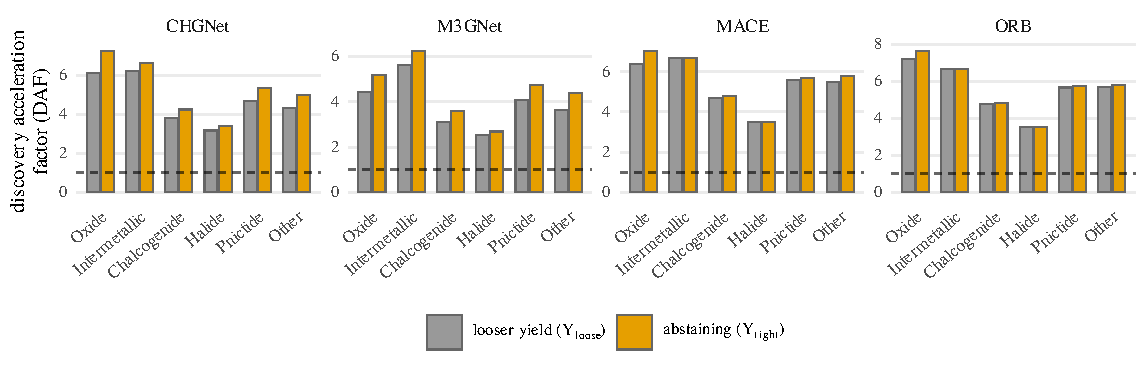
\includegraphics[width=\textwidth]{F1_daf_coverage.pdf}
  \caption{Matched-yield DAF at the looser ($Y_{\mathrm{loose}}$) and tighter
  ($Y_{\mathrm{tight}}$, abstaining) yield budgets, per anion-class stratum and per model.
  Oxides show the largest DAF lift from abstention; halides and intermetallics the smallest.}
  % source: research/results/MT29/mt29_stage1_matched_yield_result.json
  \label{fig:f1}
\end{figure}

\subsection{The stratum $\times$ coverage interaction fires, oxide-anchored and positive}

Figure~\ref{fig:f2} renders the matched-yield interaction $\mathrm{gain}_A - \mathrm{gain}_B$
for every (model, stratum-pair) cell; outlined cells have a 95\,\% bootstrap CI excluding
zero. Of the 60 cells, 48 exclude zero under an i.i.d.\ bootstrap, and all four models
% source: research/results/MT29/mt29_stage1_matched_yield_result.json (interactions_matched_yield: per-model fired chgnet 13, mace 13, m3gnet 11, orb 11; oxide-anchored 18/20; median |interaction| 0.1905)
contribute (CHGNet 13/15, MACE 13/15, M3GNet 11/15, ORB 11/15). Because WBM is generated by
elemental substitution into shared prototypes, structures sharing a parent prototype are
correlated; we therefore recompute the CIs with a prototype-blocked bootstrap that
% source: results_expansion_2026-07-11/prototype_blocked_cis/mt29_prototype_blocked_ci_result.json (blocked 45/60; shuffle 0/60; oxide-containing 17/20; chgnet ox-hal median 0.89624 CI [0.7419,1.03792]; lost cells m3gnet ox-interm, m3gnet interm-chalc, orb interm-pnict)
resamples structural-prototype clusters within each stratum (block $=$ WBM AFLOW
prototype). Under blocking 45 of 60 cells still exclude zero (the shuffle-null stays
$0/60$), and we adopt this as the primary count. The three cells that drop out are all
borderline intermetallic pairs whose i.i.d.\ CI already grazed zero (M3GNet
oxide--intermetallic and intermetallic--chalcogenide, ORB intermetallic--pnictide); no
oxide-vs-halide or strong oxide cell is affected. The firing cells are dominated by
oxide-anchored pairs: 18 of 20 oxide-containing cells fire under i.i.d.\ resampling and 17 of
20 under blocking, with oxide as the higher-benefit stratum --- a direction first observed at
Stage-1 and documented, not registered ex ante, in
a same-session Stage-2 analysis-protocol log; the general
stratum-interaction hypothesis and kill criterion were committed ex ante in
a dated pre-analysis design memo. The largest interaction is CHGNet's
oxide-vs-halide pair at $+0.90$ (prototype-blocked 95\,\% CI $[0.74, 1.04]$; i.i.d.\ CI
$[0.77, 1.04]$); the median absolute interaction across all 60 cells is $0.19$. These counts
survive formal multiplicity control
% source: research/results/MT29/mt29_multiplicity_stage1_result.json (B1000_bh_fdr_q05 46/60, hires_holm_fwer_a05 40/60, chgnet ox-hal p_holm 0.011999)
with two-sided bootstrap sign
$p$-values per cell, Benjamini--Hochberg at $q=0.05$ retains 46/60 cells (shuffle-null:
0/60), and a higher-resolution pass ($10^4$ bootstrap draws, same seed and machinery)
retains 40/60 under the stricter family-wise Holm--Bonferroni procedure at
$\alpha = 0.05$; the headline CHGNet oxide-vs-halide cell has Holm-adjusted
$p = 0.012$. The interaction is thus empirically oxide-anchored; the next subsection dissects
its mechanism directly from the predictions and finds it is driven by error-headroom and
base-rate normalization, not by hull-margin confidence being intrinsically sharper in oxide
chemistry.

\begin{figure}[t]
  \centering
  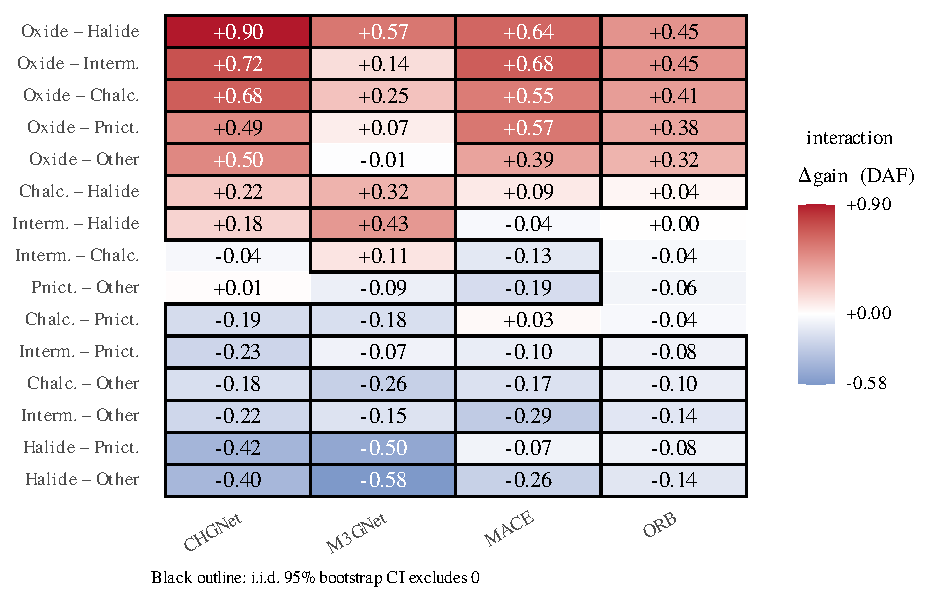
\includegraphics[width=0.82\textwidth]{F2_interaction_heatmap.pdf}
  \caption{Stratum $\times$ coverage interaction (median $\mathrm{gain}_A - \mathrm{gain}_B$)
  per model and stratum pair. Outlined cells have a 95\,\% bootstrap CI excluding zero
  (48/60 i.i.d.; 45/60 under a prototype-blocked bootstrap, the primary count --- Results).
  Oxide-anchored pairs fire positive across models.}
  % source: research/results/MT29/mt29_stage1_matched_yield_result.json
  % source: results_expansion_2026-07-11/prototype_blocked_cis/mt29_prototype_blocked_ci_result.json
  \label{fig:f2}
\end{figure}

\subsection{Mechanism: error headroom and base-rate normalization, not sharper confidence}

To test the naive reading --- that hull-margin confidence simply discriminates oxide errors
better --- we compute three post-hoc descriptive diagnostics per stratum directly from the
cached predictions (averaged over the four UIPs in Table~\ref{tab:mechanism}; full per-model
values in the reproduction archive). Two findings reframe the mechanism. First, oxides carry by
far the largest UIP formation-energy error --- RMSE $0.62$\,eV/atom versus $\sim\!0.09$ for every
other stratum --- so a large share of the structures a UIP calls stable in oxides are false
positives (called-stable precision $0.75$), leaving room for abstention to raise precision.
Second, and against the naive reading, the within-stratum rank-informativeness of the
confidence signal (AUROC of $|\hat{e}_{\mathrm{hull}}|$ separating truly-stable from
false-positive called-stable structures) is if anything the lowest of the six strata in
oxides ($0.69$ versus $0.75$--$0.78$ elsewhere): confidence does not discriminate oxide errors
better per structure. The oxide anchoring instead arises from two compounding factors --- the
large error creates the false-positive headroom, and because DAF normalizes precision by the
stratum stable base rate, which is lowest in oxides ($12.4\,\%$ versus $27.8\,\%$ for halides),
an equal precision gain from abstention becomes a larger DAF gain. These two amplifications
should be read separately, because DAF folds a genuine precision-recovery advantage together
% source: results_expansion_2026-07-10/mechanism_diag/mechanism_payoff_roster_ci.json (practitioner_payoff_chgnet: oxide precision 0.7578->0.9006 = +14.28pp, halide 0.8824->0.9481 = +6.57pp; precision-unit interaction +7.71pp; DAF gains oxide 1.1496 halide 0.2359, ratio 4.87 = 2.174 precision-recovery x 2.241 base-rate)
with the $1/\text{base-rate}$ factor. In precision-point units the CHGNet oxide-vs-halide
abstention advantage is $+7.7$ points (oxide called-stable precision lifts $+14.3$ points under
abstention, halide only $+6.6$); the headline $+0.90$ DAF interaction is that $2.2\times$
precision-recovery advantage further multiplied by DAF's $2.2\times$ base-rate denominator
(halide $27.8\,\%$ / oxide $12.4\,\%$), so the $\sim\!4.9\times$ cross-stratum DAF-gain ratio
is roughly half genuine precision headroom and half base-rate normalization. We report the
precision-unit interaction alongside DAF throughout so the base-rate amplification is transparent.
The effect is
real and reproducible --- it is exactly what the shuffle-null, LOEO, round, and
alternative-stratification controls certify --- but it is an interaction between error-driven
headroom and base-rate-normalized reporting, not evidence that a UIP is more trustworthy when
confident in oxide chemistry specifically.

\begin{table}[t]
  \centering
  \caption{Post-hoc descriptive per-stratum mechanism diagnostics, averaged over the four UIPs.
  Oxides combine the largest formation-energy error and the lowest stable base rate with ---
  against the naive reading --- the lowest confidence-rank AUROC. Base rate is the
  stratum stable fraction; RMSE is the formation-energy error; called-stable precision is the
  true-stable fraction among structures called stable; AUROC is the rank separation of
  $|\hat{e}_{\mathrm{hull}}|$ for truly-stable versus false-positive called-stable structures.}
  % source: results_expansion_2026-07-10/mechanism_diag/mechanism_payoff_roster_ci.json (mechanism_per_model_stratum + mechanism_summary: oxide base_rate 0.124, rmse 0.625, called_stable_prec 0.747, conf_auroc 0.695; per-stratum values averaged over the four legacy UIPs)
  \label{tab:mechanism}
  \begin{tabular}{lcccc}
    \toprule
    Stratum & Base rate & RMSE (eV/atom) & Called-stable prec. & Conf.\ AUROC \\
    \midrule
    Oxide          & 0.124 & 0.625 & 0.747 & 0.695 \\
    Intermetallic  & 0.142 & 0.091 & 0.631 & 0.756 \\
    Chalcogenide   & 0.205 & 0.088 & 0.725 & 0.766 \\
    Halide         & 0.278 & 0.090 & 0.752 & 0.756 \\
    Pnictide       & 0.171 & 0.097 & 0.680 & 0.775 \\
    Other          & 0.167 & 0.097 & 0.641 & 0.772 \\
    \bottomrule
  \end{tabular}
\end{table}

\paragraph{What the interaction buys a practitioner.} Concretely, for CHGNet --- the strongest
firer of the four UIPs, so this is a best-case illustration rather than a typical one --- the
% source: results_expansion_2026-07-10/mechanism_diag/mechanism_payoff_roster_ci.json (practitioner_payoff_chgnet: n_called_stable_oxide 2696, conf_half 1348, precision 0.758->0.901, daf 6.1->7.2; halide 0.882->0.948, daf 3.2->3.4)
$+0.90$ oxide-versus-halide interaction converts as follows, on the \emph{pooled} evaluation
(post-hoc descriptive, from the frozen matched-yield DAF; this pooled framing is the one that
does not transfer temporally, per Threats to validity). Of the $2{,}696$ structures CHGNet
calls stable in oxides, keeping only the
$1{,}348$ most confident by $|\hat{e}_{\mathrm{hull}}|$ raises true-stable precision from
$75.8\,\%$ to $90.1\,\%$ (DAF $6.1 \to 7.2$). A practitioner with a fixed budget of $1{,}348$
DFT relaxations therefore wastes $\sim\!134$ of them on false positives by spending it on the
confident half, versus $\sim\!326$ by spending it on a same-size random draw from all
called-stable oxides --- roughly $190$ fewer wasted relaxations. The identical abstention on
halides moves precision only $88.2\,\% \to 94.8\,\%$ (DAF $3.2 \to 3.4$; halide base DAF $3.01$,
cf.\ the provenance footnote), saving $\sim\!90$ relaxations --- about half the oxide payoff,
which is the concrete practitioner form of the interaction.

\subsection{The interaction is robust to held-out chemistry and acquisition round}

Figure~\ref{fig:f3} reports the fraction of firing cells under each robustness split.
Under LOEO, all 12 held-out-element splits remain majority-firing (12/12), pooling to
% source: research/results/MT29/mt29_stage2_robustness_result.json (gate1_loeo: drop-O 37/40 over 5 strata; min non-O split Si 39/60; gate2_rounds: 43/34/43/26/11 of 60, n_rows 40314 & 23268 for rounds 4-5)
% source: blocked_robustness_2026-07-13/mt29_blocked_downstream_ci_result.json (LOEO blocked 538/700, 12/12 splits, drop-O 36/40, shuffle 0/700; WBM-round blocked 151/300, 3/5 rounds, shuffle 0/300; committee blocked 7/15; self-validated == frozen Stage-1 blocked 45/60)
548/700 cells (538/700 under the prototype-blocked bootstrap, all 12 splits still
majority-firing); crucially, dropping oxygen --- which empties the entire oxide stratum and
leaves only 5 strata (40 cells) --- still fires 37/40 (36/40 blocked), so the effect is
not carried by
oxides alone, and no single cation or anion-former split falls below 39/60. Under the
WBM-round gate, 3 of 5 rounds are majority-firing (rounds 1--3: 43/34/43 of 60), pooling to
157/300 cells (151/300 blocked, the same 3 rounds majority-firing). Rounds 4 and 5 fall below majority (26 and 11 of 60); these are the two
smallest rounds (40k and 23k rows), so the shortfall is a per-model power effect under tiny
matched-yield budgets, not a temporal sign flip --- the oxide-highest direction is preserved
even where the CIs widen. The majority-of-splits / majority-of-rounds success criterion,
documented alongside the Stage-2 results themselves rather than registered before Stage-1,
is met on both axes.

\begin{figure}[t]
  \centering
  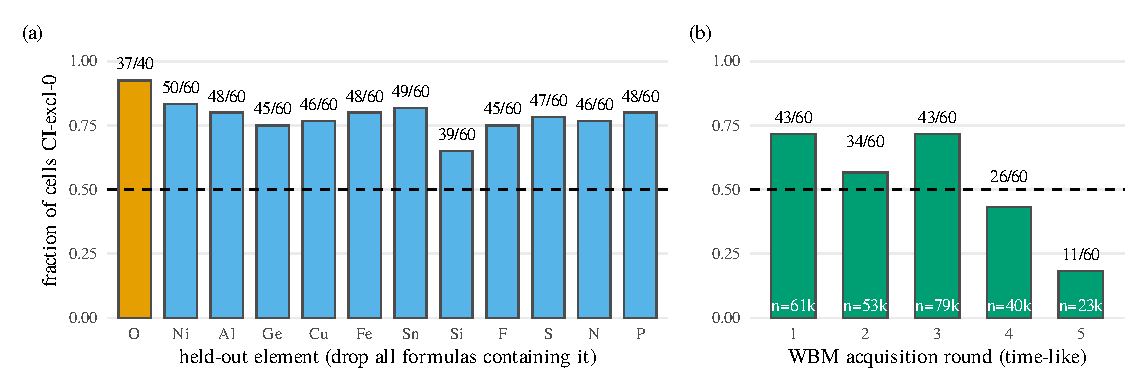
\includegraphics[width=\textwidth]{F3_robustness_panel.pdf}
  \caption{Fraction of (model $\times$ stratum-pair) cells whose 95\,\% CI excludes zero,
  per robustness split. (a) leave-one-element-out (12/12 splits majority-firing); (b)
  WBM round (3/5 rounds majority-firing). Cell counts annotated; dashed line is the majority
  threshold.}
  % source: research/results/MT29/mt29_stage2_robustness_result.json
  \label{fig:f3}
\end{figure}

\subsection{The shuffle-null is clean everywhere}

Figure~\ref{fig:f4} contrasts the magnitude of the real interaction with the
confidence-shuffled interaction, per gate. Permuting confidence within each stratum's
called-stable set collapses the signal to a tight band around zero, and no shuffled
cell's CI excludes zero in any gate: 0/60 at Stage-1, 0/700 under LOEO, and 0/300 across
% source: mt29_stage1_matched_yield_result.json (max |shuffle interaction_med| 0.00468) and mt29_stage2_robustness_result.json (shuffle 0/700, 0/300)
rounds. The largest shuffled Stage-1 interaction is $0.0047$ in absolute value, two orders
of magnitude below the real median. The interaction is therefore a property of the
confidence ordering, exactly what a genuine abstention effect requires.

\begin{figure}[t]
  \centering
  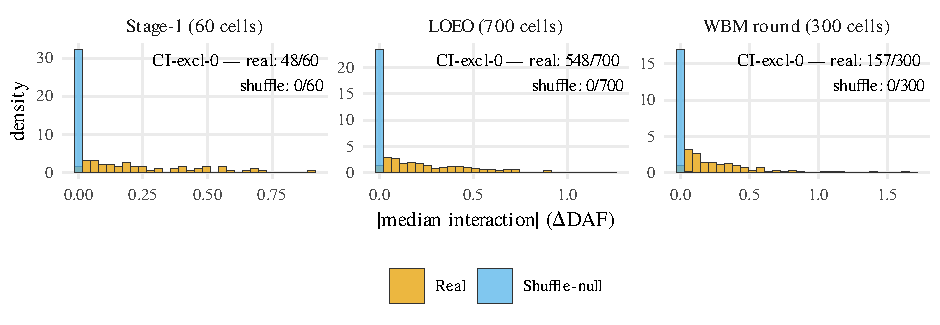
\includegraphics[width=0.82\textwidth]{F4_shuffle_null.pdf}
  \caption{Real vs.\ within-stratum confidence-shuffled $|$interaction$|$ per gate. The
  shuffle-null collapses to zero (0/60, 0/700, 0/300 cells with CI excluding zero).}
  % source: research/results/MT29/mt29_stage1_matched_yield_result.json
  % source: research/results/MT29/mt29_stage2_robustness_result.json
  \label{fig:f4}
\end{figure}

\subsection{Committee-variance abstention reproduces the interaction; native-Gaussian
coverage is optimistic in every chemistry}

Two further analyses probe whether the oxide-anchored abstention benefit is a quirk of the
particular confidence source. First, we replace each UIP's single-model
$|\hat{e}_{\mathrm{hull}}|$ with a \emph{committee-variance} signal: confidence
$=-\mathrm{std}$ of the four UIPs' reconstructed predicted hull distances, with the consensus
stable call taken as the committee-mean hull below zero, holding the matched-yield control
% source: research/results/MT29/mt29_committee_variance.json (committee_budgets y_tight 1422 / y_loose 2844; gain_median oxide 0.56329, halide -0.0139; ox-hal pair 0.57383 [0.46253, 0.68708]; chalc-hal 0.11521 [0.04381, 0.18274]; hal-pnict -0.11428 [-0.21111, -0.01857])
identical ($Y_{\mathrm{tight}} = 1422$, $Y_{\mathrm{loose}} = 2844$).
Figure~\ref{fig:f5}(a) shows the committee-variance abstention benefit is again concentrated
in oxides (matched-yield DAF gain median $+0.563$) and small elsewhere ($\le +0.10$; halide
$-0.014$). Of the 15 stratum-pair interactions, 7 have a 95\,\% bootstrap CI excluding zero
(Figure~\ref{fig:f5}(b)): all five oxide-anchored pairs positive (oxide-vs-halide $+0.574$,
CI $[0.463, 0.687]$) plus chalcogenide-vs-halide ($+0.115$, CI $[0.044, 0.183]$), with one
negative (halide-vs-pnictide $-0.114$, CI $[-0.211, -0.019]$), while the within-stratum
confidence shuffle fires 0/15. The committee's dominant interaction sign is positive,
matching the single-model reference, and it agrees in sign on all 7 jointly-significant
pairs, yet it fires far fewer pairs than the single-model consensus --- so it is a genuinely
distinct re-derivation of the effect, not a relabelling of one model. One limitation qualifies
this as \emph{corroboration} rather than independent confirmation: the committee is built from the
same four UIPs' predictions, so if those models share a correlated oxide error (plausibly through
the common MP2020-corrected labels they are trained and scored against; see Discussion), the
committee-variance signal inherits that oxide false-positive richness rather than
independently confirming it. It re-derives the interaction from a different \emph{functional} of
the same predictions, not from independent models (robustness gate verdict
PASS-BOTH; Table~\ref{tab:signalcompare}).

\begin{figure}[t]
  \centering
  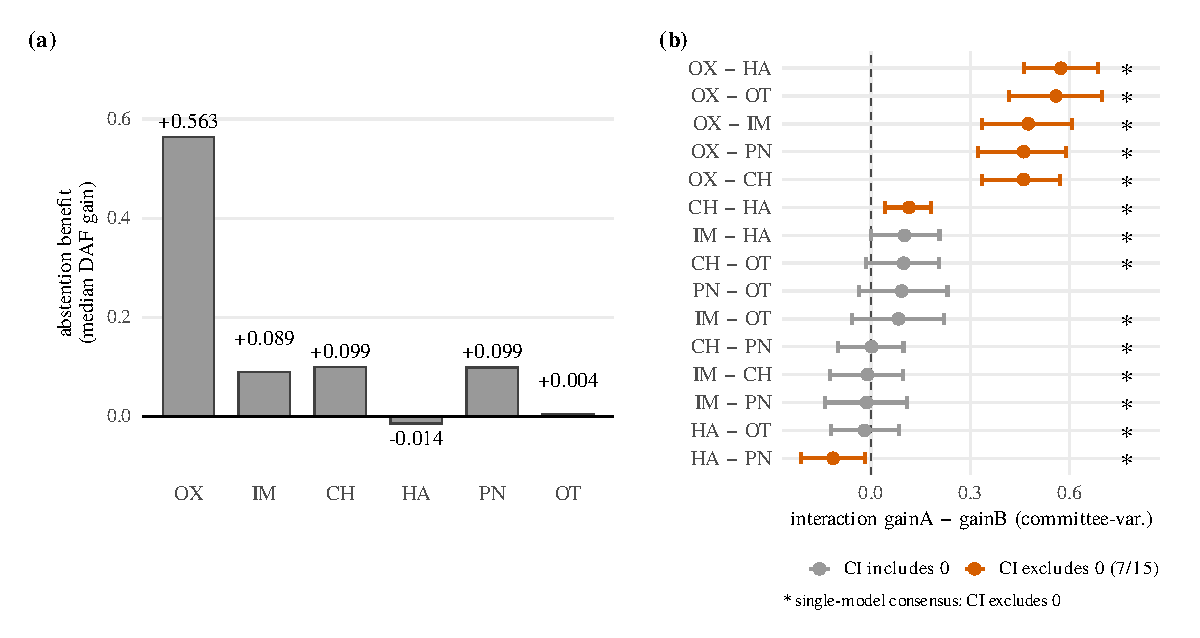
\includegraphics[width=\textwidth]{F5_committee_variance.pdf}
  \caption{Committee-variance abstention vs.\ the single-model signal. (a) Matched-yield DAF
  gain (median) per anion stratum using the committee-variance signal; the benefit
  concentrates in oxides, mirroring the single-model pattern. (b) The 15 stratum-pair
  committee-variance interactions ($\mathrm{gain}_A - \mathrm{gain}_B$, median with 95\,\%
  bootstrap CI); orange marks the 7 pairs whose committee CI excludes zero, and the side
  asterisk marks pairs on which the single-model consensus also fired. The committee is
  sparser (7/15) but sign-consistent; the confidence-shuffle collapses to 0/15.}
  % source: research/results/MT29/mt29_committee_variance.json
  \label{fig:f5}
\end{figure}

\begin{table}[t]
  \centering
  \caption{Abstention-signal comparison: the free single-model hull margin
  $|\hat{e}_{\mathrm{hull}}|$ vs.\ a four-UIP committee-variance signal, both under the
  identical matched-yield DAF control. Denominators differ because the committee collapses
  the model axis: single-model interaction cells are counted per (model $\times$
  stratum-pair) $=60$, committee interactions per stratum-pair $=15$. Both counts here use
  the i.i.d.\ bootstrap for an apples-to-apples comparison; the single-model primary count
  under the prototype-blocked bootstrap is 45/60 (Results).}
  % source: research/results/MT29/mt29_stage1_matched_yield_result.json
  % source: research/results/MT29/mt29_committee_variance.json
  \label{tab:signalcompare}
  \begin{tabular}{lcc}
    \toprule
    & Single-model $|\hat{e}_{\mathrm{hull}}|$ & Committee variance \\
    \midrule
    Confidence signal              & $|\hat{e}_{\mathrm{hull}}|$ per UIP & $-\mathrm{std}$ over 4 UIP hulls \\
    Stable call                    & predicted hull $<0$                & committee-mean hull $<0$ \\
    Matched-yield budget ($Y_{\mathrm{tight}}/Y_{\mathrm{loose}}$) & per model & $1422 / 2844$ \\
    Interaction cells CI-exclude-0 & 48/60                              & 7/15 \\
    Shuffle-null cells CI-exclude-0 & 0/60                              & 0/15 \\
    Dominant interaction sign      & $+$ (oxide-anchored)               & $+$ (oxide-anchored) \\
    Sign agreement, jointly-sig.\ pairs & ---                           & 7/7 \\
    Robustness gate verdict        & ---                                & PASS-BOTH \\
    \bottomrule
  \end{tabular}
\end{table}

Second, we ask whether a zero-free-parameter probabilistic reading of the same margin is
well-calibrated within each chemistry. Using the native Gaussian
$p_{\mathrm{stable}} = \Phi(-\hat{e}_{\mathrm{hull}}/\sigma)$, with $\sigma$ the
calibration-half RMSE of the formation-energy error, we measure the per-anion-family
conditional-coverage gap (mean $p_{\mathrm{native}}$ minus the empirical stable rate) on the
held-out test half. Every gap is positive and CI-excludes-zero for every UIP
(Table~\ref{tab:sscs}): the native Gaussian over-predicts stability in every family. The
worst-slab gap (SSCS $= \max_s |\mathrm{gap}_s|$) ranges from ORB's $0.077$ (best calibrated)
% source: research/results/MT29/mt29_sscs_stratified.json (per_model_SSCS orb 0.07684, mace 0.32176; mean 0.19737; mace sigma_rmse_cal 0.97741)
to MACE's $0.322$ (worst, driven by its inflated $\sigma = 0.977$, which pushes $p$ toward
$0.5$ everywhere), with a cross-model mean of $0.197$. Two distinct chemistry dependences must
not be conflated here. Calibration miscalibration (whether $p_{\mathrm{stable}}$ matches the
empirical stable rate) and abstention headroom (whether ranking by $|\hat{e}_{\mathrm{hull}}|$
can lift precision) are different properties: the native Gaussian is optimistic in every family,
but the stratum where it fails hardest is intermetallics for three of the four
UIPs (CHGNet, M3GNet, ORB; Table~\ref{tab:sscs}), not oxides, and only MACE has its worst
calibration gap in oxides. The abstention benefit, by contrast, is oxide-anchored for all four
models. The two axes therefore co-locate in oxides only for MACE; in general the chemistry a
UIP is least calibrated on is not the chemistry where abstention pays most.

\begin{table}[t]
  \centering
  \caption{Native-Gaussian ($p_{\mathrm{stable}} = \Phi(-\hat{e}_{\mathrm{hull}}/\sigma)$,
  zero free parameters) per-anion-family conditional-coverage gap (mean $p_{\mathrm{native}}$
  minus empirical stable rate) on the test half, per UIP. Every gap is positive and its
  95\,\% bootstrap CI excludes zero, so the native Gaussian over-predicts stability in every
  family for every model. SSCS is the worst-slab $\max_s |\mathrm{gap}_s|$.}
  % source: research/results/MT29/mt29_sscs_stratified.json
  \label{tab:sscs}
  \begin{tabular}{lcccccccc}
    \toprule
    UIP & $\sigma_{\mathrm{cal}}$ & Oxide & Interm. & Chalc. & Halide & Pnict. & Other & SSCS (worst) \\
    \midrule
    CHGNet & 0.102 & 0.109 & 0.177 & 0.139 & 0.126 & 0.148 & 0.161 & 0.177 (interm.) \\
    M3GNet & 0.117 & 0.172 & 0.214 & 0.200 & 0.177 & 0.195 & 0.207 & 0.214 (interm.) \\
    MACE   & 0.977 & 0.322 & 0.315 & 0.246 & 0.199 & 0.277 & 0.287 & 0.322 (oxide) \\
    ORB    & 0.081 & 0.074 & 0.077 & 0.048 & 0.055 & 0.038 & 0.052 & 0.077 (interm.) \\
    \midrule
    \multicolumn{8}{l}{Mean SSCS over models} & 0.197 \\
    \bottomrule
  \end{tabular}
\end{table}

\section{Discussion}

\paragraph{What the result means.} The value of selective abstention in UIP stability
screening is not uniform across chemistry, and where it is largest tracks where the reference
data is least trustworthy. At a surfaced-candidate budget held identical across
anion classes, abstaining on low-confidence calls accelerates discovery substantially more
in oxides than in halides or intermetallics --- but the load-bearing quantity is a genuine
precision advantage, not the base-rate-amplified DAF headline. Decomposed (Results,
Table~\ref{tab:mechanism}), the CHGNet oxide-vs-halide abstention gain is $+7.7$ precision
points; DAF's normalization by the low oxide base rate then amplifies that to the $+0.90$ DAF
figure, so roughly half the DAF headline is a reporting denominator and only the precision-point
interaction should be read as the effect size. The precision advantage itself does not arise
because hull-margin confidence is intrinsically sharper in oxide chemistry --- its within-oxide
rank-AUROC is if anything the lowest of the six strata --- but because oxide formation energies
are where UIP predictions disagree most with the (least trustworthy) MP2020 labels, by a wide
margin (RMSE $\sim\!0.6$ versus $\sim\!0.09$\,eV/atom elsewhere), so the largest share of oxide
stable-calls are false positives and confidence-based abstention has the most precision to
recover. Both compounding factors --- the false-positive headroom and the base-rate denominator
--- therefore point at the same place: the chemistry where the DFT reference is weakest. That is
why we read the interaction as a diagnostic of reference-data trustworthiness rather than a
chemistry-specific abstention policy. Intermetallics, by
contrast, contribute few CI-firing cells for MACE and ORB, whose intermetallic gain is
statistically indistinguishable from zero.

\paragraph{The oxide anchoring is not manufactured by WBM's construction.} A natural worry is
that the effect is an artifact of how the WBM test set is built --- elemental substitution into
known prototypes~\citep{wang2021} --- rather than a property of UIP reliability. Three features
of the analysis rule this out. First, the interaction is measured in DAF (precision normalized
by each stratum's own stable base rate) under a matched-yield control that fixes the same
absolute number of surfaced candidates in every stratum, so neither the abundance of
oxides in WBM (they are $\sim\!10\,\%$ of the joined set, not a dominant class) nor their base
rate can mechanically inflate the oxide gain --- both quantities are divided or held out.
Second, the driving quantity is the UIPs' formation-energy error, which is $\sim\!7\times$ larger
in oxides (Table~\ref{tab:mechanism}) and appears at near-identical magnitude across four
independently trained architectures; a sampling artifact of WBM would not reproduce the same
oxide-error signature across unrelated models, whereas a genuine transferability gap on oxide
chemistry would. Third, the effect survives controls that a construction artifact should not:
dropping oxygen entirely still fires the interaction ($37/40$ cells), the metal-fraction and
electronegativity stratifications --- which never reference oxide membership --- reproduce it,
and the time-like WBM-round splits preserve its direction. The oxide anchoring therefore reflects
where UIPs are least accurate, not how WBM was assembled.

\paragraph{Why UIP--label disagreement is largest in oxides --- and why the oxide labels are
least trustworthy there.} The diagnostics establish that the disagreement between a UIP's
predicted formation energy and its MP2020-corrected training label is largest in oxides
(Table~\ref{tab:mechanism}). We are careful about the level of this statement. The UIPs are
trained on the already-MP2020-corrected labels~\citep{deng2023,wang2021mp2020}, so their
residual is a model fitting error on corrected targets, not a leakage of the semilocal-DFT
(GGA) error into the prediction --- that GGA error lives in the labels and is corrected before the
model ever sees it. Two documented properties of universal potentials make oxides the hardest
chemistry to fit: a systematic potential-energy-surface softening / energy underprediction shared
across uMLIP architectures~\citep{deng2025softening}, and a per-chemistry error concentration in
oxide and transition-metal chemistry reported in independent
assessments~\citep{yu2024assessment}. The MP2020 corrections are themselves
composition- and oxidation-state-dependent step functions~\citep{wang2021mp2020} that a smooth
interatomic potential is ill-suited to reproduce, which plausibly amplifies the oxide fitting gap
(the anomalously large oxide formation-energy RMSE in Table~\ref{tab:mechanism}, several times the
models' aggregate error, is consistent with such a hard-to-fit seam and is not separately
isolated here). Compounding this, the oxide labels are also the least reliable slice of the
ground truth: correlated-$d$ transition-metal oxides require a Hubbard-$U$ treatment that the
PBE-based Materials Project reference does not consistently carry~\citep{wang2006oxidation,
jain2011formation}, and the very existence of the MP2020 anion/oxidation-state corrections is a
symptom that oxide DFT energetics carry uncorrected seams. Two things therefore co-locate in
oxides --- the chemistry a UIP fits worst, and the chemistry whose reference energies are least
trustworthy --- and our disagreement metric cannot separate them. The abstention benefit is
present in main-group oxides too (Table~\ref{tab:tmoxide}), so it is not carried by the
correlated-$d$ sub-family alone; but we do not claim to have isolated a single physical cause. The
demonstrated result remains the two-factor account of the abstention benefit above (error headroom
$\times$ base-rate normalization), now read as headroom in UIP--label disagreement rather
than in UIP error against a trusted truth.

\paragraph{The oxide benefit is not a transition-metal-oxide artifact.} Splitting the oxide
stratum into transition-metal oxides (formula containing a $d$-block metal; $17{,}369$ structures)
and main-group oxides ($7{,}651$) shows the matched-yield abstention benefit is present in
both sub-families for all four UIPs (Table~\ref{tab:tmoxide}): keeping the more-confident
half of each sub-family's called-stable structures gives a positive DAF gain in every
(model, sub-family) cell. Main-group oxides, which lack the transition-metal $d$-electron
localization seam, show a comparable benefit, so the effect is not carried by transition-metal
oxides alone --- consistent with the anion-level (oxygen) DFT correction being the broad driver of
the oxide error (post-hoc descriptive; full values in the reproduction archive).

\begin{table}[t]
  \centering
  \caption{Within-oxide split (post-hoc descriptive): matched-yield abstention detail for
  transition-metal oxides ($n=17{,}369$) versus main-group oxides ($n=7{,}651$), per UIP.
  $n$ called-stable is the sub-family's called-stable count at the loose budget; precision is
  the true-stable fraction among called-stable structures, full budget $\to$ confident half.
  DAF gain is positive in all eight cells.}
  % source: results_expansion_2026-07-11/mechanism_extensions/m3_prospective_m4_within_oxide.json (M4_within_oxide: n_tm_oxide 17369, n_maingroup_oxide 7651; per_model.{chgnet,m3gnet,mace,orb}.{tm_oxide,maingroup_oxide}: n_called_stable, precision_full, precision_conf_half, daf_gain; both_subfamilies_positive 4/4)
  \label{tab:tmoxide}
  \begin{tabular}{llccc}
    \toprule
    UIP & Sub-family & $n$ called-stable & Precision (full$\to$half) & DAF gain \\
    \midrule
    CHGNet & TM-oxide    & 1778 & $0.771\to0.917$ & $+1.24$ \\
           & Main-group  & 918  & $0.733\to0.867$ & $+0.97$ \\
    M3GNet & TM-oxide    & 2907 & $0.512\to0.579$ & $+0.56$ \\
           & Main-group  & 1292 & $0.632\to0.785$ & $+1.11$ \\
    MACE   & TM-oxide    & 2221 & $0.757\to0.825$ & $+0.58$ \\
           & Main-group  & 1047 & $0.860\to0.973$ & $+0.83$ \\
    ORB    & TM-oxide    & 2003 & $0.878\to0.950$ & $+0.61$ \\
           & Main-group  & 962  & $0.922\to0.938$ & $+0.11$ \\
    \bottomrule
  \end{tabular}
\end{table}

\paragraph{What DFT verification would and would not add.} A natural question for a screening
paper is whether any prediction was verified against density-functional theory. For this audit the
question is answered by construction: the estimand throughout is agreement with WBM's
MP2020-compatible DFT ground truth~\citep{wang2021mp2020,riebesell2025}. Every structure a UIP
calls stable, every abstention, and every stable/unstable flip is scored against an
already-computed DFT hull distance, so the precision, DAF, and coverage numbers are
DFT-referenced by definition. Running new DFT on the flipped or abstained candidates would not
test any claim made here; it would test the fidelity of the WBM ground truth itself, which is
upstream of our contribution and shared by every Matbench Discovery result. We therefore run no
new DFT, and none is required for the audit's validity: unlike a discovery study that must confirm
novel predictions, our claims are statements about decision behavior measured against DFT labels
% source: reference-reliability caveat --- correlated-d TM-oxide labels lacking Hubbard-U in the PBE MP reference (wang2006oxidation, jain2011formation); full statement given once above ("Why UIP--label disagreement...") and cross-referenced here (de-duplicated in the 2026-07-16 revision)
that already exist. One caveat follows directly, and bounds the oxide reading: because the
estimand is agreement with those labels, the audit inherits their reliability, and --- as
established above (``Why UIP--label disagreement is largest in oxides'') --- the oxide labels are
the benchmark's least reliable slice of the ground truth. The oxide-anchored abstention benefit is therefore anchored to the slice of
WBM where the ground truth is weakest, so the finding is best read as ``UIP--label disagreement is
largest, and least trustworthy, in oxides,'' not as a certified statement about UIP error against
a fully trusted truth. This does not affect the non-oxide interactions or the method itself, only
the interpretation of the oxide anchor. To be explicit, our claims are statements about decision
behavior measured against DFT labels
that already exist.

\paragraph{Why this survives where the ``beats margin'' wedge did not.} The companion study
tested whether a learned or calibrated confidence signal (isotonic $p_{\mathrm{stable}}$,
cross-model disagreement) beats hull margin at matched coverage and matched stable-call
yield, and found that none did (0/12 cells): margin was undefeated, not shown insufficient. The
present result does not contradict that; it asks a different, orthogonal question --- whether
margin's own well-established abstention benefit is uniform across chemistry, and finds it is
not. Pooling oxides (large benefit) with intermetallics (no benefit) at matched yield washes
the average out, so the signal lives in the interaction across anion strata, not in a
main-effect claim about whether margin beats some other baseline, which is why it survives
the same common-absolute-yield control that companion study used. We carried that control
through genuine anion-class strata, leave-one-element-out, and WBM-round splits, and it survives
all of them with a clean shuffle-null.

\paragraph{Relation to certified and ensemble-uncertainty approaches.} Two adjacent
literatures address confidence for UIPs, but neither reports a chemistry-conditioned value of
abstention. Proof-Carrying Materials~\citep{pcm2026} delivers a global, non-stratified
risk-of-failure model (AUC-ROC $0.938$) backed by formal safety certificates --- a
calibration/certification contribution, not a stratum $\times$ coverage DAF interaction, and
it reports no chemistry-conditioned abstention benefit. Multi-head-committee ensemble
uncertainty~\citep{beck2025} instead constructs a richer confidence signal (committee-of-heads
prediction standard deviation) and validates it via force-error correlation and
active-learning data efficiency; it neither uses the free $|\hat{e}_{\mathrm{hull}}|$ baseline
nor tests whether the value of any confidence signal for stability screening varies by
chemistry. Recent calibration-focused work on UIP uncertainty --- flexible post-hoc
calibration~\citep{ho2026flexcalib} and uncertainty quantification for \emph{misspecified}
potentials~\citep{perez2025uqmisspec} --- sharpens the confidence estimate itself but likewise
does not condition the value of abstention on chemistry. Closest in framing,
PROBE~\citep{probe2026} recasts UIP reliability as
\emph{selective classification} via a post-hoc probe on frozen representations, but does so at
the per-atom level during molecular dynamics rather than at the WBM stability decision, and
reports no chemistry-conditioned value of abstention. The present work is orthogonal to all
three: it is deliberately agnostic to the source
of the confidence signal --- the oxide-anchored interaction persists whether the signal is the
cheapest single-model $|\hat{e}_{\mathrm{hull}}|$ or a four-model committee variance
(Figure~\ref{fig:f5}, Table~\ref{tab:signalcompare}) --- and isolates a stratum-dependent
abstention benefit that neither the certification nor the ensemble-uncertainty literature
reports. Within Digital Discovery, \citet{yu2026uaal} similarly probes the reliability
limits of uncertainty-aware screening --- there, uncertainty-guided active learning for
lead-free halide perovskites, where the confidence signal recurrently flags heavy $d$-electron
halides as likely functional-driven false positives. Our matched-yield audit occupies the same
reliability-of-screening lane at benchmark scale ($32$ UIPs, $\sim$257k structures): rather than
choosing which candidates to acquire, it asks whether the value of abstaining is itself
chemistry-dependent, and --- consistent with that work's caution about chemistry-localised
failure --- finds its largest payoff precisely in the oxide stratum.

\paragraph{Statistical-rigor and reproducibility precedent within Digital Discovery.} The
audit-protocol framing here --- a frozen, provenance-gated re-analysis of already-published
prediction files rather than a new trained model --- has direct precedent in this journal's own
methodology literature. Persaud et al.~\citep{persaud2024reproducibility} show that even a single
published materials-ML result can fail to reproduce without careful provenance tracking, the
failure mode our md5-gated, byte-identical reproduction is built to rule out. Ottomano
et al.~\citep{ottomano2024aggregation} show that a common materials-informatics assumption ---
that aggregating more training data uniformly helps --- does not survive a matched, controlled
comparison, the same matched-yield discipline this paper applies to abstention rather than to
training-set size. Witman and Schindler's {MatFold}~\citep{witman2025matfold} standardizes
cross-validation splitting for materials-discovery models precisely because naive splits bias
performance estimates, echoing why this paper reports LOEO and WBM-round splits as robustness
gates rather than a single held-out number. On the confidence-signal side, a Digital Discovery
perspective on uncertainty in ML atomistic modeling~\citep{grasselli2025uncertainty} surveys
Bayesian and ensembling UQ approaches broadly, and architecture-search-based ensembling for
molecular-property UQ~\citep{jiang2024autognnuq} offers a richer alternative confidence signal in
the same spirit as the committee-variance comparison here (Figure~\ref{fig:f5}); neither reports a
chemistry-conditioned abstention value, the gap this paper fills.

\paragraph{Scope and what stays dead.} We claim an abstention-quality interaction at
matched yield, read as a diagnostic of where the reference data is least trustworthy --- and
nothing beyond that diagnostic. The positive deliverable is that reading, not a forward-looking
policy: stratification does not re-order the four models' overall
stability-screening performance --- the rank-reordering framing tested earlier remains dead ---
we do not assert per-round significance for every model, and (per Threats to validity and the
falsified knapsack) we do not claim a deployable stratum-targeting allocator. The two under-powered WBM
rounds (4 and 5) are reported transparently as a power limitation concentrated in the weakest
firer (ORB), not as evidence of temporal decay.

\paragraph{Fixed-hull recompute: validated.} The predicted hull distance used throughout is
the fixed-hull reconstruction $\hat{e}_{\mathrm{hull}} = e_{\mathrm{hull}}^{\mathrm{true}} +
(\hat{e}_{\mathrm{form}} - e_{\mathrm{form}}^{\mathrm{true}})$, which holds the true convex hull
fixed and moves only by the model's formation-energy error. We validate this shortcut against a
from-scratch convex-hull recompute off the Materials Project phase diagram on a stratified
$5{,}000$-structure subset ($4{,}998$ evaluated). Once the MP reference surface is placed on the
same MP2020-corrected formation-energy convention as the query (the correction layer that built
the ground-truth column; a first execution mistakenly used total DFT energies, and its
implausible multi-eV apparent deltas were what flagged the mismatch --- a useful audit tell,
since the delta $\hat{e}_{\mathrm{hull}}^{\mathrm{fixed}} - \hat{e}_{\mathrm{hull}}^{\mathrm{recomp}}$
is model-independent by construction, so a large value can only be a reference bug), the recompute
reproduces the published $e_{\mathrm{above\,hull}}$ to $\sim\!10^{-3}$\,eV/atom in every stratum
(per-stratum mean $|\Delta| \le 0.0009$) and changes the stable/unstable call for only
$13$ of $4{,}998$ structures ($0.26\,\%$; CHGNet 5, M3GNet 6, MACE 1, ORB 1). Those $13$ flips
are confined to the mixed-anion strata (halide 5, pnictide 4, chalcogenide 3, other 1), with
zero in oxide and zero in intermetallic --- so the two strata that anchor the
headline interaction are exactly where the fixed-hull call is most stable. One scoping caveat:
this recompute certifies the fixed-hull \emph{reconstruction} --- that recomputing
$e_{\mathrm{above\,hull}}$ from each model's predicted formation energy against the true Materials
Project reference set reproduces the shortcut --- and not the deeper approximation that the
competing phases defining the hull are themselves unmoved by a UIP's errors on those
phases (every reference entry here is DFT ground truth, not a UIP prediction). The stability
calls the paper actually uses are the reconstructed ones, and it is those that are validated: the
fixed-hull approximation is a sound basis for the stability calls throughout, not merely an
acknowledged limitation.

\paragraph{Roster-wide universality of the oxide anchor.} The four-UIP headline rests on
cached predictions that carry the MP2020 corrections natively. To test whether the oxide
anchoring is a property of those four models or of universal potentials as a class, we converted
every credential-free WBM prediction file on the Matbench Discovery Figshare record
(version~25): $44$ files --- $27$ trained on Materials Project~\citep{jain2013mp} data only (the
2022--24 ``MP generation,'' including seven 2020-era classical baselines) and $17$ trained on the
newer OMat24~\citep{barrosoluque2024omat24} / Alexandria~\citep{schmidt2023alexandria} / OpenLAM
corpora (the ``OMat generation''). Each file's MP2020-corrected
formation-energy column is the authoritative published prediction --- byte-identical to the
frozen CHGNet anchor over all $256{,}963$ rows --- so the expansion sits on the same ground truth
as the headline, not a re-derivation. All $44$ raw sources were re-verified against their
Figshare-published md5 checksums (an automated verification pass, $44/44$ OK). The roster and
its two-arm generational aggregation follow a pre-specified analysis plan written before the
run; it is not
git-timestamped ahead of the run, unlike the alternative-stratification plan below, so we label it
a pre-specified plan rather than a preregistration.

\emph{Model families represented in the roster.} Beyond the four headline architectures already
introduced --- CHGNet~\citep{deng2023}, M3GNet~\citep{chen2022}, MACE~\citep{batatia2022mace}
(here the MACE-MP-0 foundation checkpoint~\citep{batatia2024macemp0}), and ORB~\citep{neumann2024}
--- the $32$-model roster (Table~\ref{tab:roster}) spans several further architecture families:
message-passing equivariant networks (NequIP~\citep{nequip2022}, its strictly local variant
Allegro~\citep{allegro2023}, and the equivariant transformer EquiformerV2~\citep{liao2024equiformerv2}),
the graph-generalized atomic cluster expansion family (GRACE~\citep{grace2024}), the DPA line of
large atomic models (DPA-2~\citep{zhang2024dpa2} and DPA-3~\citep{zhang2025dpa3}), and two recent
smooth/local-frame potentials (eSEN~\citep{fu2025esen} and AlphaNet~\citep{yin2025alphanet}),
alongside MatterSim~\citep{yang2024mattersim}, Orb-v3~\citep{rhodes2025orbv3}, and
SevenNet~\citep{park2024sevennet,sevennet} introduced above. The oxide anchor's universality
across this architecturally diverse set (Table~\ref{tab:roster}) is part of what licenses reading
it as a property of universal potentials broadly rather than of any one model family.

\emph{One published file is a non-independent duplicate.} Of the $44$ converted files, the
OMat-generation Orb-v2 file (Figshare file 51607307,
``orbff-v2-20241011.csv.gz'') is byte-identical (max\,$|\Delta e_{\mathrm{form}}| = 0$ over all
$256{,}963$ rows) to the frozen \textsc{MP}-generation ``orb'' headline anchor: both trace to the
same published Orb-v2 checkpoint. The frozen anchor had been labelled ``Orb-v2 MPtrj-only,'' but
re-fetching and cross-checking both published Orb-v2 files shows the anchor matches the general
Orb-v2 checkpoint (file 51607307) exactly and the true MPtrj-only checkpoint (file 51607310,
``orbff-mptrj-only-v2-20241014.csv.gz'') only approximately (mean\,$|\Delta| = 0.037$,
max\,$|\Delta| = 1.99$\,eV/atom). This file is therefore excluded from the
generational contrast as a non-independent duplicate rather than an additional OMat-generation
model, leaving $43$ independent models. This is a labelling/duplication issue, not a corrupt or
fabricated file: its md5 gate passes cleanly, and it is the only one of the $44$ sources that is
non-independent.

\emph{Correction to the earlier Orb-v3 ``dissenter'' claim.} A previous version of this check
self-inferred predictions for a four-model roster and reported Orb-v3 as a sharp oxide-anchoring
reversal ($-1.83$). That figure was an artifact of the self-inference, which omitted
the MP2020 anion/oxide corrections and thereby imprinted a systematic anion-count-proportional
offset ($\approx\!+0.11$--$0.59$\,eV/atom, largest on oxides) that the ground truth and the cached
CSVs both carry, leaving the reconstructed-hull oxide calls degenerate. On the \emph{authoritative
published} Figshare v25 predictions, Orb-v3's oxide-vs-halide abstention interaction is $+0.64$
(95\,\% CI $[0.52, 0.76]$) --- positive and oxide-anchored like every other modern potential. We
correct the earlier reversal explicitly: it was a harness artifact, not a model property.

\emph{The oxide anchor is universal across the modern-UIP roster.} Under the pre-specified
inclusion rule ($\ge\!50$ called-stable structures per stratum and $\ge\!99\%$ WBM coverage, which
keeps the common-yield budget non-degenerate), $32$ modern UIPs qualify ($16$ MP-generation, $16$
OMat-generation, after dropping the duplicate). The oxide-vs-halide matched-yield interaction is
positive with a prototype-blocked 95\,\% CI excluding zero for all $32$ ($16/16$
MP-generation, $16/16$ OMat-generation), and oxide is the single highest-benefit stratum in
$29/32$ (the three exceptions are MP-generation models whose arg-max is the residual ``other''
stratum, not a reversal); per-model interactions range from $+0.31$ to $+1.31$
(Table~\ref{tab:roster}). The pre-specified hypothesis that the newer OMat generation would
dissolve or reverse the anchoring is not supported: a model-level permutation test on the
generation label gives $p = 0.68$ (observed MP$-$OMat gap in mean interaction $-0.037$, 95\,\% CI
$[-0.21, 0.13]$; $n_{\mathrm{MP}} = 16$, $n_{\mathrm{OMat}} = 16$). We read this as no detectable
generational difference in the oxide anchor: the CI is wide relative to the observed gap and the
analysis is underpowered (at $n=16$ per arm) to exclude a moderate-magnitude generational shift,
so ``generation-independent'' should be read as an honest null within this roster's power, not as
a demonstrated invariance.

\emph{Classical baselines and multiplicity.} The seven 2020-era classical baselines (CGCNN,
CGCNN+P, MEGNet, Wrenformer, Voronoi-RF, ALIGNN, BOWSR-MEGNet; all MP-trained) are by contrast weak
and mixed --- five carry a positive CI-excluding oxide-vs-halide interaction but oxide is the
arg-max stratum for only two, and Voronoi-RF reverses it ($-0.12$, CI $[-0.22, -0.02]$) ---
so the effect is specific to modern universal potentials, not shared by every ML formation-energy
model. Over the full included-UIP interaction family ($32 \times 15 = 480$ cells) $378$ CI-exclude
zero and $369$ survive Benjamini--Hochberg FDR~\citep{benjamini1995fdr} at $q = 0.05$; the
oxide-vs-halide subfamily is $32/32$ under both, with a clean within-stratum confidence-shuffle
null ($0/480$). The Holm--Bonferroni family-wise procedure~\citep{holm1979}
survives $0/480$ (and $0/32$ on the oxide-halide subfamily) at $\alpha = 0.05$: this is a
bootstrap-resolution limit, not evidence against the effect --- the minimum achievable two-sided
bootstrap $p$ at $n_{\mathrm{boot}} = 1000$ is $\approx\!0.002$, and Holm's family-wise correction
over $480$ (or $32$) cells demands $p < 0.05/480 \approx 1.0\times10^{-4}$ (or $0.05/32
\approx 1.6\times10^{-3}$), both below the achievable floor; the BH-FDR and raw-CI readings above
are the informative ones here, mirroring the treatment of the equivalent Stage-1 Holm result.
Numbers trace to
% source: results_expansion_2026-07-14/mt29_roster_expansion_result.json (n_included_uip 32; MP_arm n 16 n_positive_anchored 16 n_argmax_oxide 13; OMat_arm n 16 n_positive_anchored 16 n_argmax_oxide 16; V3 perm_p 0.68153 gap -0.03708 CI [-0.2083,0.13303]; multiplicity_full_family n 480 ci_excl0 378 bh 369 holm 0; multiplicity_oxide_halide 32/32 holm 0; shuffle_null 0/480; orb_v3 ox-hal 0.6426 CI [0.52029,0.75598]; classical voronoi_rf -0.11704 CI [-0.21828,-0.01686])
the roster-expansion audit in the reproduction archive
(the corrected re-run; supersedes the contaminated
earlier run, retained with a provenance note).

\emph{Two published files with non-physical MAE, retained with disclosure.} Two MP-generation files
as published on Figshare v25 --- GRACE-2L-MPtrj and SevenNet-0 --- contain a handful of
catastrophic-outlier prediction rows ($13$ and $1$ of $256{,}963$, with $|\hat{e}_{\mathrm{form}}|$
up to $10^{22}$ and $10^{33}$\,eV/atom) that make their naive mean absolute error
non-physical ($5\times10^{16}$ and $10^{28}$\,eV/atom); trimming those rows restores physical MAEs
of $0.057$ and $0.046$\,eV/atom. Because the analysis ranks and thresholds predictions rather than
averaging them, these rows do not affect the result: removing them shifts each oxide-vs-halide
interaction by $\le\!0.013$ (well inside its $\sim\!0.3$-wide CI) and leaves the arg-max stratum and
CI-exclusion unchanged, so both models are retained among the $32$ with this disclosure rather than
silently trimmed.
% source: results_expansion_2026-07-13/DATA-SANITY-OUTLIERS.json (grace_2l_mptrj 13 rows mae_naive 5.28e16 mae_trimmed 0.05719 delta_I 0.01325; sevennet_0 1 row mae_naive 9.60e27 mae_trimmed 0.04642 delta_I 0.00194; both robust True; unaffected by the orb_v2_omat dedup, both MP-generation models)

\emph{Frozen-anchor provenance disclosure.} Three of the four headline anchors (M3GNet, MACE-MP-0,
and the ``orb'' anchor discussed above) are frozen on-disk snapshots that are not the
current Figshare v25 publication: cross-checking each against its re-downloaded v25 counterpart
shows measured drift (mean\,/\,max absolute difference in eV/atom: M3GNet $0.036$/$3.65$;
MACE-MP-0 $0.050$/$349.59$; orb $0.037$/$1.99$; CHGNet is byte-identical, $0$/$0$). The drift does
not change any reported number --- the four-UIP headline and the roster expansion both use the
frozen snapshots (or, for orb, the published file the snapshot equals) consistently, and the drift
magnitudes are disclosed here for provenance rather than folded into any statistic.
% source: results_expansion_2026-07-13/ROSTER25_DATA_MANIFEST.json (anchor_crosscheck: chgnet identical; m3gnet mean_abs 0.03582 max_abs 3.6457; mace_mp_0 mean_abs 0.04955 max_abs 349.5859; orb_mptrj mean_abs 0.03721 max_abs 1.994)

\begin{table}[t]
  \centering
  \small
  \caption{Roster-wide oxide-vs-halide matched-yield abstention interaction $I$ (prototype-blocked
  95\,\% CI) for all $32$ included modern UIPs, by training generation (models are Matbench
  Discovery leaderboard identifiers; the published Orb-v2
  OMat file is excluded here as a non-independent duplicate of the MP-generation ``orb'' anchor,
  text). $I>0$ with CI excluding zero for all $32$; oxide is the highest-benefit stratum in $29$.
  GRACE-2L-MPtrj and SevenNet-0 carry non-physical published MAE from a few outlier rows that do
  not affect this rank-based interaction (text).}
  \label{tab:roster}
  % source: results_expansion_2026-07-14/mt29_roster_expansion_result.json (per_model oxide|halide interaction_med + ci95, all 32 included UIPs, sorted by I within generation)
  \begin{tabular}{lcc@{\hskip 1.4em}lcc}
    \toprule
    \multicolumn{3}{c}{MP generation ($n=16$)} & \multicolumn{3}{c}{OMat generation ($n=16$)} \\
    \cmidrule(lr){1-3}\cmidrule(lr){4-6}
    model & $I$ & 95\,\% CI & model & $I$ & 95\,\% CI \\
    \midrule
    eqv2\_s\_mp & $+1.16$ & $[1.02,1.29]$ & allegro\_oam & $+1.31$ & $[1.19,1.44]$ \\
    matris\_mptrj & $+1.01$ & $[0.88,1.13]$ & dpa31\_ft & $+1.13$ & $[1.00,1.25]$ \\
    dpa3\_v2\_mptrj & $+0.99$ & $[0.86,1.13]$ & dpa3\_v2\_openlam & $+0.98$ & $[0.86,1.11]$ \\
    allegro\_mp & $+0.95$ & $[0.80,1.11]$ & grace\_1l\_oam & $+0.91$ & $[0.77,1.04]$ \\
    grace\_2l\_mptrj & $+0.91$ & $[0.76,1.06]$ & eqv2\_m\_omat & $+0.90$ & $[0.77,1.03]$ \\
    mattersim & $+0.83$ & $[0.71,0.94]$ & dpa3\_v1\_openlam & $+0.83$ & $[0.71,0.96]$ \\
    dpa3\_v1\_mptrj & $+0.83$ & $[0.70,0.95]$ & alphanet\_oma & $+0.70$ & $[0.58,0.82]$ \\
    hienet & $+0.74$ & $[0.60,0.87]$ & esen\_oam & $+0.70$ & $[0.58,0.81]$ \\
    nequip\_mp & $+0.59$ & $[0.45,0.73]$ & nequip\_oam\_xl & $+0.67$ & $[0.55,0.77]$ \\
    matris\_10m\_mp & $+0.58$ & $[0.47,0.69]$ & orb\_v3 & $+0.64$ & $[0.52,0.76]$ \\
    eqnorm\_mptrj & $+0.50$ & $[0.37,0.63]$ & mace\_mpa & $+0.62$ & $[0.48,0.75]$ \\
    alphanet\_mp & $+0.49$ & $[0.37,0.61]$ & grace\_3l\_oam & $+0.57$ & $[0.45,0.67]$ \\
    sevennet\_0 & $+0.48$ & $[0.34,0.61]$ & grace\_2l\_oam & $+0.55$ & $[0.44,0.68]$ \\
    nequix\_mp & $+0.42$ & $[0.29,0.57]$ & nequip\_oam & $+0.54$ & $[0.42,0.64]$ \\
    sevennet\_l3i5 & $+0.41$ & $[0.27,0.55]$ & matris\_oam & $+0.50$ & $[0.40,0.61]$ \\
    esen\_mp & $+0.38$ & $[0.25,0.52]$ & grace\_2l\_oam\_l & $+0.31$ & $[0.19,0.42]$ \\
    \bottomrule
  \end{tabular}
\end{table}

\paragraph{Threats to validity.} The primary confound is surfaced-candidate yield, addressed
by the common-absolute-yield budget. Stratum-definition sensitivity is probed two ways, both of
which survive: by the LOEO of the anion-formers (F, S, N, P) and the drop-oxygen run, and ---
directly addressing the ``cherry-picked stratifier'' objection --- by re-running the entire
matched-yield interaction under two alternative stratum definitions that do not use the
anion-priority ordering, preregistered ex ante and git-timestamped (2026-07-02 10:52\,UTC,
% prereg commit 66f078c precedes result commit 2eeddcd (git-verifiable ex-ante ordering)
before the analysis runs at 11:01\,UTC): amount-weighted mean-Pauling-
electronegativity quintiles and amount-weighted metal-fraction bins. Both reproduce the
chemistry-dependence (overall verdict \textsc{both\_robust}):
% source: research/results/MT29/mt29_altstrat_multiplicity_result.json (per_stratifier_verdict EN q5 SUCCESS, metal_fraction SUCCESS, overall BOTH_ROBUST, BH-across-families 18/80)
the interaction CI-excludes zero in
% source: mt29_stage1_altstrat_electronegativity_q5_result.json (ci_excl0 31/40, shuffle 0/40) and mt29_stage1_altstrat_metal_fraction_result.json (ci_excl0 24/40, shuffle 0/40)
$31/40$ (electronegativity) and $24/40$ (metal-fraction) model~$\times$~stratum-pair cells, with
the more anion-/oxide-rich, less-metallic strata carrying the higher abstention benefit. We are
% source: mt29_stage1_altstrat_electronegativity_q5_result.json (ci_above0_correct_direction 6/40); mt29_stage1_altstrat_metal_fraction_result.json (ci_above0_correct_direction 14/40)
careful not to overstate the electronegativity stratifier as a clean anti-cherry-pick rebuttal:
of its $31$ CI-excluding cells only $6/40$ fire \emph{in the hypothesized anion-rich$>$metal-rich
direction} (the rest exclude zero in mixed or opposite directions, because its top quintile pools
oxides and halides --- opposite-extreme anion classes), whereas metal-fraction reproduces the
direction cleanly ($14/40$ in-direction). It is therefore metal-fraction, not electronegativity,
that provides the clean directional reproduction. Both nonetheless survive within-family Holm
correction ($5$ and $13$ anion-consistent survivors, Holm-adjusted
$p$ down to $8.0\times10^{-3}$) with a clean shuffle-null ($0/40$ each). Metal-fraction is
cleanly monotonic (mf1, nonmetal-rich, highest benefit; mf5, $96\,\%$ intermetallic, lowest);
the electronegativity quintiles confirm the heterogeneity but are non-monotonic at the top
quintile for a chemically sensible reason --- it pools oxides and halides, the two
opposite-extreme anion classes --- reported transparently in a dedicated
% source: findings-altstrat-2026-07-02.md
alternative-stratification findings note. The chemistry-dependence is therefore not an artifact
of the single anion-priority classification rule.
Thin-stratum DAF instability is guarded by minimum-row and minimum-called-stable thresholds.
Multiple comparisons are handled three ways: by requiring a majority of cells rather
than any single cell, by pairing every real test with a matched shuffle-null (zero false
positives observed), and by a formal correction: per-cell two-sided bootstrap sign
% source: research/results/MT29/mt29_multiplicity_stage1_result.json and mt29_multiplicity_stage2_result.json (BH 46/60, 539/700, 135/300; Holm hires 40/60; shuffle 0/60, 0/700, 0/300)
$p$-values with Benjamini--Hochberg at $q = 0.05$ applied within each family retain 46/60
Stage-1, 539/700 LOEO, and 135/300 WBM-round cells (shuffle families: 0/60, 0/700, 0/300),
and the family-wise Holm--Bonferroni procedure at $\alpha = 0.05$ retains 40/60 Stage-1
cells in a higher-resolution $10^4$-bootstrap pass (Holm is bootstrap-resolution-limited at
$m = 700/300$ with $10^3$ draws, so BH-FDR is the formal correction reported for the
robustness families). One structural caveat applies to all of these corrections: within a model
the $15$ stratum-pair contrasts are not independent --- with six strata they span only
five independent dimensions, since any pair difference is fixed by the others (e.g.\
$(\mathrm{oxide}-\mathrm{halide}) = (\mathrm{oxide}-\mathrm{intermetallic}) -
(\mathrm{halide}-\mathrm{intermetallic})$). BH and Holm treat the linked contrasts as separate
tests, so the effective number of independent stratum comparisons is five per model, not fifteen;
the corrected counts should be read with that redundancy in mind. Every reproduced cell in these correction runs was asserted
identical (median, CI, exclusion status) to the frozen Stage-1/Stage-2 result JSONs before
$p$-values were attached. The single confidence signal $|\hat{e}_{\mathrm{hull}}|$ is the free
hull-margin baseline; richer signals such as cross-model ensemble disagreement are future work.
The companion study's audit found disagreement does not survive the joint
matched-coverage-and-yield control and can underperform margin there (e.g.\ CHGNet
% source: research/results/MT28/mt28_riskcov_result.json (chgnet/by_coverage/cov_50/disagree/matched_yield_gain -0.0724)
cov\_50 matched-yield gain $-0.0724$, 95\,\% CI $[-0.0845, -0.0610]$, excluding zero in the
negative direction), so whether a richer signal would strengthen or dilute the stratified
interaction is an open question, not an assumed one. The tight/loose yield split itself
($Y_{\mathrm{tight}} = Y_{\mathrm{loose}} // 2$) was fixed once, post hoc; a subsequent
sensitivity sweep re-ran the identical matched-yield machinery at
$Y_{\mathrm{tight}} = \mathrm{round}(Y_{\mathrm{loose}} \cdot r)$ for
$r \in \{1/3, 0.4, 0.5, 0.6\}$ (same seed, same 1000-bootstrap CIs). The interaction count is
% source: research/results/MT29/mt29_stage1_yield_ratio_sensitivity_result.json (excl0_by_ratio 45/47/48/47 of 60; chgnet ox-hal medians 1.14417, 0.99069, 0.90092, 0.75099)
stable across the grid --- 45/60, 47/60, 48/60, and 47/60 cells CI-excluding zero at
$r = 1/3, 0.4, 0.5, 0.6$ respectively, with the shuffle-null clean (0/60) at every ratio ---
and the headline CHGNet oxide-vs-halide cell fires at all four ratios (median interaction
$+1.14$, $+0.99$, $+0.90$, $+0.75$; monotone in $r$ as expected, since a looser tight budget
dilutes the abstention contrast). The ratio choice is therefore a confirmed non-issue for
the qualitative claim, though the interaction magnitude scales with the budget ratio.
A prospective, temporally held-out check calibrates the stratified-abstention policy on early
WBM acquisition rounds and applies it to later rounds; it shows the oxide-highest
ordering does not transfer out-of-time, and we report both specifications
% source: results_expansion_2026-07-11/mechanism_extensions/m3_pooled.json (calib 1-3, apply 4+5: oxide positive 4/4 but oxide_top_gain 0/4, oxide_beats_other_mean 0/4, verdict MIXED) and m3_prospective_m4_within_oxide.json (round-5-only: orb future_oxide_daf_gain -0.001, oxide beats mean 2/4, top 0/4)
per the forking-paths rule under which the arm was run. In the primary pooled specification
(calibrate rounds 1--3, apply to the pooled later rounds 4--5), the oxide abstention benefit
stays positive for all four UIPs but is the top-benefit stratum for none (0/4)
and falls below the mean of the other strata for all four (0/4 beat the
other-strata mean; overall verdict \textsc{mixed}); the high-benefit strata out-of-time are
intermetallics and pnictides. In the round-5-only sensitivity specification (calibrate rounds
1--4, apply to round 5) the picture is weaker still: ORB's future-round oxide gain is
marginally negative ($-0.001$) and oxide beats the other-strata mean for only 2 of 4
models. The oxide-anchored ordering is therefore a property of the pooled evaluation
and does not survive a prospective, temporally held-out test; whether a stratified policy
should target oxides in deployment is consequently not established here.

\paragraph{Next step --- and a caution on turning the interaction into an allocator.} The
tempting policy reading --- ``spend the abstention budget preferentially on oxide candidates
rather than applying a uniform global confidence cutoff'' --- does not follow
automatically, and our own follow-up falsified its strongest form. A constrained greedy
knapsack allocator that reallocates a fixed total-coverage budget across strata by marginal
DAF (coverage $0.7$, seed 20260629, 1000-bootstrap CIs) failed to CI-dominate the global
threshold on per-stratum DAF:
% source: research/results/MT29/mt29_b5b_knapsack_constrained-exec-2026-06-29.json (summary: positive_excl0 5, negative_excl0 14 of 24; aggregate positive models 0/4; verdict FALSIFIED-NO-DOMINANCE)
of 24 (model $\times$ stratum) cells, 5 improved with CI excluding zero but 14 worsened
with CI excluding zero, and the equal-weight aggregate mean DAF improved with CI excluding
zero in 0 of 4 models. The mechanism is a conservation constraint: at matched total coverage,
per-stratum DAF depends only on that stratum's kept count, so any reallocation is zero-sum
across strata --- what oxides gain, other strata give back. The interaction documented here
therefore licenses stratified reporting and stratified expectations (which chemistries
a confidence cutoff will actually help, and by how much), and it licenses spending
additional abstention capacity where it pays, but it does not license reshuffling a
fixed budget away from a global threshold. The alternative-stratification robustness reported
above (Threats to validity) already addresses the stratifier-choice objection directly; a
richer-confidence comparison remains for a benchmarks-track submission.

\section*{Data and code availability}

All inputs are the public Matbench Discovery~\citep{riebesell2025} on-disk cached artifacts
(WBM summary ground truth from~\citep{wang2021} and the four cached UIP
prediction CSVs); no authentication or run-time download is required. The genuine ex-ante
commitment --- the general strata direction and kill criteria --- is a dated pre-analysis
design memo (written before Stage-1; committed to the version-controlled repository
in the pre-push baseline, with the other previously-untracked frozen artifacts). The
Stage-2 analysis-protocol log is, by its own disclosure, a same-session analysis protocol and
results log rather than an ex-ante preregistration: it records that the exact success thresholds
and budget parameters were fixed during the Stage-1/Stage-2 runs themselves. The one
preregistration with a git-verifiable ex-ante ordering is the alternative-stratification prereg,
whose commit precedes its result commit (see Threats to validity).
% ex-ante artifacts: DEEP-REVERIFY-2026-06-21.md (committed 2026-07-02, commit c7a036b); same-session Stage-2 log research/results/MT29/prereg-stage2-mt29-2026-06-22.md; alt-strat prereg commit 66f078c precedes result commit 2eeddcd
% frozen result JSONs (research/results/MT29/ unless noted): mt29_stage1_matched_yield_result.json; mt29_stage2_robustness_result.json; mt29_stage1_yield_ratio_sensitivity_result.json; mt29_multiplicity_stage1_result.json; mt29_multiplicity_stage2_result.json; mt29_b5b_knapsack_constrained-exec-2026-06-29.json; mt29_stage1_altstrat_electronegativity_q5_result.json; mt29_stage1_altstrat_metal_fraction_result.json; mt29_altstrat_multiplicity_result.json; results_expansion_2026-07-10/corrected_arms/{mt29_hull_recompute_corrected_result.json,mt29_stage1_oam_arm_corrected_result.json}; results_expansion_2026-07-11/prototype_blocked_cis/mt29_prototype_blocked_ci_result.json (block=protostructure_spglib); results_expansion_2026-07-11/mechanism_extensions/{m3_prospective_m4_within_oxide.json,m3_pooled.json}; results_expansion_2026-07-10/mechanism_diag/mechanism_payoff_roster_ci.json; results_expansion_2026-07-14/{mt29_roster_expansion_result.json,mt29_roster_expansion_manifest.json,verify_roster_md5.py} + results_expansion_2026-07-13/{ROSTER25_DATA_MANIFEST.json,DATA-SANITY-OUTLIERS.json} (44 published-potential files converted, 43 independent models / 32 included UIPs after dropping the orb_v2_omat duplicate; pre-specified plan mt29_roster_expansion_PREREG-2026-07-13.md, dated 2026-07-13, not git-timestamped ahead of the run; supersedes the contaminated results_expansion_2026-07-13/mt29_roster_expansion_result.json, retained with a CONTAMINATED-2026-07-14.md provenance note)
The frozen
results are the Stage-1 matched-yield interaction/shuffle-null record and the Stage-2
LOEO/WBM-round robustness record, each with a SHA-256 manifest over inputs, script, and output.
Supplementary frozen records cover the budget-ratio sweep, the formal multiple-comparison
correction, the falsified stratum-aware allocator, the two alternative-stratification robustness
runs with their cross-stratifier multiplicity summary, and the corrected insurance arms (the
fixed-hull validation and the modern-roster reproduction), each with its own manifest. The
prototype-blocked Stage-1 CIs resample WBM AFLOW prototype clusters, and the mechanism-extension
post-hoc diagnostics --- the within-oxide transition-metal/main-group split
(Table~\ref{tab:tmoxide}) and the prospective temporal-transfer specifications (pooled and
round-5-only; Table~\ref{tab:mechanism} and the practitioner payoff) --- are each labelled post-hoc descriptive. % figure scripts: manuscripts/figures/F1_daf_coverage.R ... F5_committee_variance.R (portfolio paper-template pattern); retired duplicate pipelines under manuscripts/archive/
The code is developed at GitHub (\url{https://github.com/PeterPonyu/materials-mlip-research}) and
archived at Zenodo under DOI \texttt{10.5281/zenodo.21130295}; this DOI is currently reserved on a
draft deposition and becomes active when the record is published.
A single self-contained figure
pipeline --- one R/ggplot2 script per figure, following the shared portfolio
paper-template pattern --- reads those frozen result records directly and regenerates every
figure; no value in this paper is hand-entered. (Two earlier figure pipelines were quarantined
after an audit found a duplicated R and matplotlib pipeline silently overwriting
each other's outputs; the present single R pipeline supersedes both.)
\paragraph{Licensing, compute, and packaging.} The entire data-and-model chain is
license-clean with no non-commercial clause (Table~\ref{tab:licenses}). All analysis --- including
the roster expansion ($44$ published-potential files, $43$ independent models) --- is CPU/pandas
only and reads published,
credential-free Matbench Discovery predictions (no network access, tokens, or model weights at run
time). A superseded earlier arm self-inferred four models on a single RTX 4090D (24\,GB; measured
peak GPU memory $6.3$\,GiB, peak utilisation $84\,\%$ over the $256{,}963$-structure pass, per-minute
\texttt{nvidia-smi} log); it is retained only as the diagnostic that surfaced the MP2020-omission
artifact corrected in the roster analysis above, and contributes no reported number.

\begin{table}[t]
  \centering
  \caption{License provenance for the data and models. No component carries a
  non-commercial (CC-BY-NC) restriction.}
  \label{tab:licenses}
  \begin{tabular}{lll}
    \toprule
    Component & Role & License \\
    \midrule
    WBM test set~\citep{wang2021}          & ground-truth stability & CC-BY-4.0 \\
    Matbench Discovery code~\citep{riebesell2025} & benchmark/eval harness & MIT \\
    MACE / MACE-MP-0~\citep{batatia2022mace} & UIP (code + checkpoint) & MIT \\
    MatterSim~\citep{yang2024mattersim}     & UIP (code + checkpoint) & MIT \\
    Orb-v3~\citep{rhodes2025orbv3}          & UIP (code + weights)   & Apache-2.0 \\
    SevenNet-MF-ompa~\citep{park2024sevennet,sevennet} & UIP (code + checkpoint, $\ge$0.12.0) & MIT \\
    \bottomrule
  \end{tabular}
\end{table}

\paragraph{Reproducibility-chain status (self-reported).} Both Stage-1 and Stage-2 have now
been independently re-executed on CPU from the same on-disk cached inputs and
their manifests regenerated against the current scripts. The Stage-1 manifest
reproduced its frozen output
byte-for-byte identical across two independent
re-runs in different Python/numpy/pandas environments. The Stage-2 manifest, whose recorded script hash had previously
gone stale relative to the on-disk Stage-2 analysis script (the script file was
touched after the manifest was first generated), was regenerated by this re-run: the script
hash now matches the on-disk script, and the frozen output again reproduced byte-for-byte
identical, confirming the Stage-2 result is
genuinely deterministic and unaffected by the earlier hash staleness. The
analysis scripts, frozen result records, manifests, figure scripts, and this manuscript are
committed to a version-controlled GitHub repository
(\url{https://github.com/PeterPonyu/materials-mlip-research}) and archived at Zenodo under
DOI~\texttt{10.5281/zenodo.21130295}, following the baseline GitHub-plus-Zenodo archiving
pattern and Digital Discovery's requirement of a DOI-bearing archive alongside the actively
maintained development mirror. The GitHub repository is private during peer review (a
portfolio-wide precaution against scooping) and will be made public on acceptance; the Zenodo
DOI is currently reserved on a draft deposition and becomes active on publication.

% Bibliography via natbib/BibTeX (shared-template pattern): shared.bib is the
% portfolio bibliography copied in by `make bib`; refs.bib holds the
% paper-specific entries (keys disjoint from shared.bib).
\bibliographystyle{plainnat}
\bibliography{shared,refs}

\end{document}
